\documentclass[tikz,border=4pt]{standalone}
% Estilo común de los diagramas de bloques (se usa con \input en cada standalone)
\usepackage[defaultsans,scale=0.92]{lato}
\usepackage{libertinust1math}
\usepackage{xcolor,amsmath}
\usepackage{tikz}
\usetikzlibrary{positioning,arrows.meta,calc,shapes.geometric}
\usepackage{../../notacion}
\definecolor{ctrlazul}{HTML}{1E5AA8}\definecolor{ctrlnoche}{HTML}{14213D}
\definecolor{ctrlcoral}{HTML}{D1495B}\definecolor{ctrlverde}{HTML}{2A9D8F}
\definecolor{ctrlambar}{HTML}{E09F3E}\definecolor{ctrlgris}{HTML}{5C677D}
\definecolor{ctrlvioleta}{HTML}{6C4AB6}\definecolor{ctrlteal}{HTML}{0F7173}
\tikzset{
  >={Stealth[length=2.4mm]}, every node/.style={font=\small},
  bloque/.style={draw=ctrlnoche,fill=ctrlazul!7,thick,rounded corners=1.5pt,minimum height=9mm,minimum width=13mm,inner sep=4pt},
  suma/.style={draw=ctrlnoche,thick,circle,inner sep=0pt,minimum size=6mm},
  senal/.style={->,thick,draw=ctrlnoche},
  rot/.style={font=\footnotesize,text=ctrlgris},
}

\begin{document}
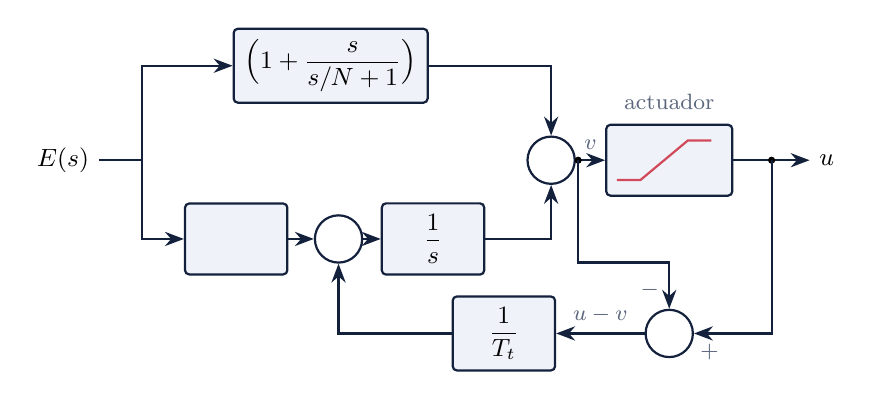
\begin{tikzpicture}
  \node (e) at (0,0) {$E(s)$};
  \coordinate (e0) at (1.0,0);
  \node[bloque] (PD) at (3.4,1.2) {$\Kc\Big(1+\dfrac{\Td s}{\Td s/N+1}\Big)$};
  \node[bloque] (Ki) at (2.2,-1.0) {$\dfrac{\Kc}{\Ti}$};
  \node[suma] (S1) at (3.5,-1.0) {};
  \node[bloque] (In) at (4.7,-1.0) {$\dfrac{1}{s}$};
  \node[suma] (S2) at (6.2,0) {};
  \node[bloque,minimum width=16mm] (Sat) at (7.7,0) {};
  \draw[thick,ctrlcoral] ($(Sat.west)+(1.5mm,-2.5mm)$) -- ++(3mm,0) -- ++(6mm,5mm) -- ++(3mm,0);
  \coordinate (u0) at (9.0,0);
  \node (u) at (9.7,0) {$u$};
  \node[suma] (S3) at (7.7,-2.2) {};
  \node[bloque] (Tt) at (5.6,-2.2) {$\dfrac{1}{T_t}$};
  \draw[thick,draw=ctrlnoche] (e) -- (e0);
  \draw[senal] (e0) |- (PD);
  \draw[senal] (e0) |- (Ki);
  \draw[senal] (Ki) -- (S1);
  \draw[senal] (S1) -- (In);
  \draw[senal] (In) -| (S2);
  \draw[senal] (PD) -| (S2);
  \draw[senal] (S2) -- node[above,rot]{$v$} (Sat);
  \draw[senal] (Sat) -- (u);
  \fill (u0) circle (1.3pt);
  \draw[senal] (u0) |- node[pos=0.9,below,rot]{$+$} (S3);
  \coordinate (vv) at ($(S2)!0.5!(Sat.west)$); \fill (vv) circle (1.3pt);
  \draw[senal] (vv) |- ($(S3)+(-8mm,9mm)$) -| node[pos=0.8,left,rot]{$-$} (S3);
  \draw[senal] (S3) -- node[above,rot]{$u-v$} (Tt);
  \draw[senal] (Tt) -| (S1);
  \node[rot,above=0.5mm of Sat] {actuador};
\end{tikzpicture}
\end{document}
